\documentclass[a4paper,conference]{IEEEtran}

\IEEEoverridecommandlockouts
%\usepackage{hyperref}
\usepackage{url}
\usepackage[utf8]{inputenc}
\usepackage[T1]{fontenc}
\usepackage[cmex10]{amsmath}
\usepackage{balance}
\usepackage{subfig}
\usepackage {graphicx}
\usepackage{amssymb}

\title{Improving Predictive Entry of Finnish Text Messages using IRC Logs}


% author names and affiliations
% use a multiple column layout for up to three different
% affiliations
\author{
\IEEEauthorblockA{\ldots\\
\ldots\\
\ldots\\
\ldots}
\and
\IEEEauthorblockA{\ldots\\
\ldots\\
\ldots\\
\ldots}
\and
\IEEEauthorblockA{\ldots\\
\ldots\\
\ldots\\
\ldots}
}



\begin{document}



%\IEEEspecialpapernotice{(Authors' pre-print draft version)}
\maketitle


\begin{abstract}
We describe a predictive text entry system for Finnish combining an
open source morphological analyzer Omorfi and a lexical model compiled
from Internet Relay Chat (IRC) logs. The system is implemented as a
weighted finite-state transducer (WFST) using the freely available
WFST library HFST. We show that using IRC logs to train the system
gives substantial improvement in recall from a baseline system using
word frequencies computed from the Finnish Wikipedia. We evaluate our
system against the predictive text entry systems in three widely
available mobile phone models and establish that we achieve comparable
recall.
\end{abstract}

\section{Introduction}
\label{sec:introduction}

\IEEEPARstart{M}{obile} phone text messages are a hugely popular way
of communication, but mobile phones are not especially well suited for
inputting text because of their small size and often limited
keyboard. There are several technological solutions for inputting text
on mobile phones and other limited keyboard devices. This paper is
concerned with a technology called predictive text entry, which utilizes
redundancy in natural language in order to enable efficient text entry
using limited keyboards (typically having 12 keys).

There has been a lot of research into improving predictive text entry,
but it has mainly been concerned with improving the statistical model,
or other technical aspects of text entry such as the keyboard
layout. In this paper, we investigate the what role the training data,
used in constructing the predictive text entry system, plays on the
recall.

Ideally the training data for any data driven system, such as
predictive text entry, should resemble the input data of the system as
closely as possible. In the case of a predictive text entry system,
the ideal training data would thus consist of text messages. Since
text messages are difficult to come by and there are legal
restrictions for using them, other sources for training data should be
considered.

In this paper, we use Internet Relay Chat (IRC) logs, to train a
predictive text input system for Finnish. In IRC multiple users chat
in public chat rooms and often these conversations are logged and the
logs are posted on the Internet. We show that using IRC logs as
training data gives significant improvement compared to a baseline
system, which is trained using data from the Finnish Wikipedia.

To the best of our knowledge, there have not been earlier inquiries
into using IRC logs for training predictive text entry systems. IRC
log material is nevertheless very well suited for the task, since
there is a lot of material available in different languages. Like text
messages, it resembles spoken language and typically consists of short
messages of a couple of hundred of characters.

We evaluate our system against the predictive text entry in a number
of widely available mobile phones (Nokia 9200, Nokia C7 and Samsung
SGH-M310) and show that we achieve comparable recall. This
demonstrates that it is possible to construct an accurate predictive
text entry system without resorting to actual text message data. Even
estimating the parameters of the system can be accomplished without
using actual text message data.

Because Finnish is a morphologically complex language, our system uses
a morphological analyzer for Finnish Omorfi
\cite{pirinen/2011/nodalida} rather than simply using a word list. The
word forms found in Omorfi are given probabilities according to their
frequency in the Finnish Wikipedia. These probabilities are combined
using similar probabilities computed from IRC logs and the final
probability given for a word form is a combination of the
probabilities given by Omorfi and the IRC log model.

Since Omorfi is implemented as a weighted finite-state transducer
(WFST), we implemented our predictive text entry system in the
weighted finite-state framework. We used HFST
\cite{conf/sfcm/Linden2009}, a freely available open-source C++
interface, for constructing and utilizing WFSTs.

This paper is organized as follows: In section \ref{sec:related-work},
we present earlier work in improving the recall of predictive text
entry systems. In section \ref{sec:text-entry}, we present the predictive
text entry task. In section \ref{sec:methods}, we explain how to
augment a morphological analyzer with word frequencies computed from
IRC logs and how such a system is used to disambiguate between
suggestions corresponding to an ambiguous input sequence. After this
we present the morphological analyzer, Omorfi, and the HFST interface
in section \ref{sec:tools} and present the IRC log data used for
training out model and the text message data used for evaluation in
\ref{sec:data}. We evaluate our system in section \ref{sec:evaluation}
and present some general and closing remarks in sections
\ref{sec:discussion} and \ref{sec:conclusions}.

% - Demonstrate the relevance of the research problem.
%   * Predictive text entry works poorly, because it doesn't adequately take 
%     into account the difference between general written language and text 
%     messages.
%   * We need more realistic training data.
%   * Genuine text messages are hard to come by.
% - Instead of text messages, we use IRC logs, which can easily be harvested
%   from the internet (from the public domain?) and which ressemble text 
%   messages.
% - We claim that using IRC Logs and a dictionary we can achieve significant 
%   improvement compared to using only a morphological dictionary
% - We demonstrate that IRC logs can be used to both train and weight a 
%   predictive text entry system for text messages withput resorting to 
%   text message data even for adjusting the weights of component models.
%   (something like that...) 
% - To the best of our knowledge there have been no previous published
%   using IRC logs to train predictive text entry systems.

\section{Related Work}
\label{sec:related-work}

Improving predictive text entry is a widely researched problem. The
improvements can be divided into two broad categories (i) improving
the statistical model used in predictive text entry by e.g. using
context dependent models or improving the training material and (ii)
improving the design of the keypad of the mobile phone in order to
support faster typing.

Ganslandt \& al. \cite{ganslandt/2009} and Gong \&
al. \cite{gong/2008} have extended the statistical model by
incorporating context into the model. They use both traditional word
bigrams and more complex syntactic and semantic contextual
restrictions. Gong \& al. additionally use a POS tagger as part of the
model.

E.g. How and Kan \cite{how05optimizing} and Bellman and Mackenzie
\cite{Department98aprobabilistic} have researched ways to reorder
letters on the mobile phone keypad in order to make typing more
efficient. The model of Bellman and Mackenzie is adaptive.

We are concerned with improving the statistical model by using
training data that resembles text messages. Using genre or
domain-specific text to train an NLP system is not a new idea and it
has also been applied to predictive text entry. Harbusch \&
al. \cite{Harbusch/2003} investigate the usefulness of a
domain-specific lexical model in predictive text entry. They establish
that it is difficult to assemble a good enough purely domain-specific
lexical model. According to them, the best approach is therefore to use a
combination of a high coverage general lexical model and a domain-specific
model, which is exactly what we have done.

The work by Harbusch \& al. is closely related to our own work, but they
are concerned with building systems for very specific domains such as
school exercises and scientific texts. They do not really address the
question of what would constitute practical training material for a
general text message system. We are expressly interested in improving
entry of text messages using widely available materials (namely IRC logs).

There has also been work on using finite-state transducers for
predictive text entry. Forcada \cite{Forcada01corpus-basedstochastic} uses
stochastic (i.e. weighted) finite-state transducers to construct a
predictive text entry system for Catalan and our model is similar to
theirs, but their system works with a word-list, whereas our system
uses a morphological analyzer.  In addition our system allows for
merging lexical models from several sources.
 
\section{Predictive Text Entry}
\label{sec:text-entry}

The keypad of a typical mobile phone has twelve keys for typing
numbers and symbols. Additionally there are function keys, which are
used for various other purposes. The typical layout uses ten keys for
typing numbers. Nine of those are also used for typing letters (including
<SPACE>). The remaining two keys are used for typing special symbols,
e.g. "*", "\#" and "+". Figure \ref{fig:keypad} shows a typical layout
for a mobile phone keyboard.

The letters of the English alphabet are distributed between the keys
from 2 to 9, in such a way that each key can be used to type three or
four letters. The key 0 is used to type <SPACE>.

For most languages whose alphabet differs from the English alphabet,
number keys are also used to input those symbols, which are
not found in the English alphabet. E.g. the three Finnish letters not
found in the English alphabet "å'', "\"{a}" and "\"{o}" are typed
using key 2 in case of "å" and "\"{a}" and key 6 in case of "\"{o}".

Since each key from 2 to 9 corresponds to at least three different
letters, every sequence of numbers encodes many different letter
sequences. We call the letter sequences {\it suggestions}. Predictive
text entry is the task of finding the correct suggestion corresponding
to the number sequence received as input from a user of the mobile
phone. The correct suggestion is the letter sequence the user
intended, typically a word.

Our method is based on lexical models derived from different
sources. In this paper we consider the problem of disambiguating
between suggestions, which have been encoded in the lexical
models. Thus we do not consider the problem of finding the correct
suggestion for number sequences which cannot correspond to any of the
words encoded in the lexical models or finding other suggestions besides
those that have been encoded in the lexical models. Neither do we
consider the problem of finding the correct suggestion based on
partial input.

\begin{figure}
\begin{center}
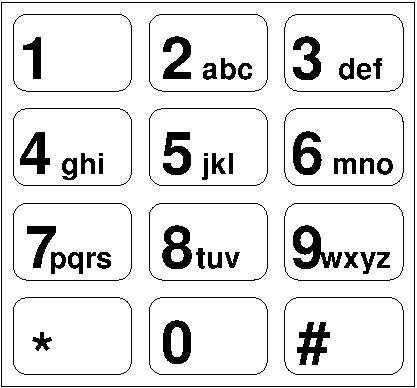
\includegraphics[width=1.5in]{keypad.pdf}
\end{center}
\caption{The layout of a typical twelve-key mobile phone keyboard.}
\label{fig:keypad}
\end{figure}

\section{Methods}
\label{sec:methods}

Our predictive text entry system is based on probabilistic lexical
models of the Finnish language. By a lexical model, we mean a model,
which assigns some probability between 0 and 1 to the words in a
language.

We first construct two probabilistic lexical models of Finnish,
using an existing Finnish morphological analyzer Omorfi and IRC logs, and combine
them to achieve a model of Finnish which (i) has broad lexical
coverage and (ii) gives a good approximation of the probabilities of
word forms in text messages. We then transform the model so that it
can be used as a machine, which takes number sequences such as "2452"
as input.

Our model outputs a list of suggestions that correspond to the number
sequence given as input. The list contains only suggestions, which
have been encoded in the lexical models, so if the correct suggestion
is not found in the lexical models, our method cannot suggest it. The
suggestions are appended with a probability, which is computed by
combining the probabilities given by the lexical models used to
construct the model. The suggestions are given to the user in order of
decreasing probability. The list of suggestions corresponding to
"2452" could contain e.g. "aika" and "äijä".

We have chosen to implement our system using {\it weighted finite-state
transducers} (WFST), partly because the morphological analyzer Omorfi is
implemented as a WFST, but also because they provide a flexible way of
combining models to build language technology applications.

\subsection{Weighted Finite-State Transducers}

%The weighted language model in our finite-state language model is based
%on morphological dictionary of the language created in traditional
%finite-state morphology framework\cite{beesley/2003}. The weights in
%this system will be basic scaled unigram weights transformed in
%finite-state form by $w = -\log \frac{f}{cs}$ where $w$ is the weight,
%$f$ is the frequency of token and $cs$ the size of corpus in
%tokens. For tokens that do not exist maximum weight of $w_{max} =
%-\log \frac{1}{cs+1}$ is used.  The probabilities are gained by
%extracting the word frequencies from a large scale corpus such as
%wikipedia~\cite{pirinen/2010/lrec}. The basic unigram weighting system
%can be fine-tuned, especially on part of unknown words, by composing
%additional weights based on e.g. morphological complexity, as
%suggested in \cite{karlsson/1992}, which can be easily modeled in
%weighted finite-state form as suggested e.g. in\cite{schiller/2005}

Finite-state transducers are a class of computational models, which
rewrite input strings to output strings \cite{beesley/2003}. The input
string $s_i$ and its output string $s_o$ are called a correspondence
and written $s_i\mathrm{:}s_o$. If $T$ is a transducer, we write
$s_i\mathrm{:}s_o \in T$, iff $T$ rewrites $s_i$ to $s_o$, i.e. {\it
  accepts} the correspondence $s_i\mathrm{:}s_o$. If $T$ accepts an
identity correspondence $s\mathrm{:}s$, we say that $T$ accepts the
string $s$.

Morphological analyzers are classical examples of language
technological applications implemented as finite-state
transducers. They rewrite input words e.g. "dog" to sets of
morphological analyses $\{$"dog+NOUN+SG", "dog+VERB+INF"$\}$. Here
"dog" is the input string in two correspondences "dog":"dog+NOUN+SG"
and "dog":"dog+VERB+INF".

Our system is implemented using weighted finite-state transducers
(WFSTs). These are an extension of finite-state transducers, where
every correspondence $s_i\mathrm{:}s_o$ between an input string $s_i$
and an output string $s_o$ receives a {\it weight} $\mathrm{w}_T(s_i\mathrm{:}s_o)$. Here $T$ is the transducer. The weight is a floating point number. 

The weights in our system represent probabilities, which have been
transformed into so called {\it penalty weights} using the map $p
\mapsto -\log p$. Probabilities are transformed into penalty weights
in order to avoid underflow in computer arithmetics. 

Since the probability $0$ corresponds to an infinite penalty weight,
we say that a transducer $T$ gives infinite weight to correspondences
it doesn't accept. Weight arithmetics is approximate probability
arithmetics, taking into account the transformation $p \mapsto -\log
p$. Addition of weights $w_1 \oplus w_2$ corresponds to taking their
minimum $\min(\{w_1,w_2\})$ and multiplication $w_1 \otimes w_2$
corresponds to ordinary addition of floating point numbers $w_1 +
w_2$. The addition operation $\oplus$ underestimates the penalty
weight of the sum of the underlying probabilities $-\log (e^{-w_1} +
e^{-w_2})$, but the approximation is usually good enough.

Akin to ordinary transducers, WFSTs can be combined using
different binary algebraic operations or modified using unary
algebraic operations to yield new WFSTs. Our system uses two unary and three binary operations:
\begin{itemize}
\item {\bf Projection $\mathrm{P}(T)$:} A unary operation, whose result
  rewrites a string $s_i$ to itself, iff the argument rewrites $s_i$
  to some output string $s_o$. The weight given to each correspondence
  $s_i:s_i$ is
  \begin{equation}
    \bigoplus_{s_i\mathrm{:}s_o \in T} \mathrm{w}_T(s_i\mathrm{:}s_o)
  \end{equation}
\item {\bf scaling $\mathrm{W}_k(T)$, where $k \in \mathbb{R}$:} A unary operation, whose result accepts the same correspondences $s_i\mathrm{:}s_o$ as $T$ with weight $k\cdot \mathrm{w}_T(s_i\mathrm{:}s_o)$. Here we use regular multiplication of floating point numbers (not $\otimes$).\footnote{Actually scaling is of course a set of unary operations. One for each floating point number $k$.}
\item {\bf Disjunction $S \cup T$:} (sometimes called union) A binary
  operation, whose result rewrites an input strings $s_i$ to the
  output string $s_o$, iff one of the argument transducers writes
  $s_i$ to $s_o$. The weight given each correspondence
  $s_i\mathrm{:}s_o$ is
  \begin{equation}
    \mathrm{w}_S(s_i\mathrm{:}s_o) \oplus \mathrm{w}_T(s_i\mathrm{:}s_o)
  \end{equation}
\item {\bf composition $S \circ T$:} A binary operation, whose result
  writes an input string $s_i$ into an output string $s_o$, iff the
  first argument rewrites $s_i$ to some string $t$ and the second
  argument rewrites $t$ to $s_o$. The weight given each correspondence
  $s_i\mathrm{:}s_o$ is
  \begin{equation}
    \bigoplus_{s_i\mathrm{:}t \in S, t\mathrm{:}s_o \in T} \mathrm{w}_S(s_i\mathrm{:}t) \otimes \mathrm{w}_T(t\mathrm{:}s_o)
    \end{equation}
\item {\bf Subtraction $S - T$:} A binary operation whose result accepts those correspondences in $S$, which are not accepted by $T$. The weight remains the same, so
  \begin{equation}
    \mathrm{w}_{S-T}(s_i\mathrm{:}s_o) < \infty \Rightarrow \mathrm{w}_{S-T}(s_i\mathrm{:}s_o) = \mathrm{w}_{S}(s_i\mathrm{:}s_o)
  \end{equation}
\end{itemize}
For a more thorough discussion on WFSTs, see Allauzen \& al. \cite{openfst/2007}.

\subsection{Components of the predictive text entry system}

Our system is constructed from three WFSTs, which are combined using
disjunction, subtraction and composition:

\begin{itemize}
\item A transducer $[\mathrm{Num}\rightarrow\mathrm{Text}]$, which
  rewrites number sequences to letter sequences like a 12-key mobile phone
  works. E.g. $[\mathrm{Num}\rightarrow\mathrm{Text}]$ would rewrite
  $23$ to the strings "ad", "ae", "af", "bd", "be", "bf", "cd", "ce"
  and "cf". Each correspondence in $[\mathrm{Num}\rightarrow\mathrm{Text}]$
  receives equal weight.
\item A lexical model transducer $L_O$, which rewrites word forms to
  themselves (i.e. gives an identity correspondence) and associates a
  penalty weight corresponding to a probability to known word
  forms. The probability is based on corpus frequencies. An English
  lexical model might e.g. accept the correspondence "be":"be" with penalty
  weight $5.41$ corresponding to the probability $0.39\%$.
\item A domain specific lexical model transducer $L_I$, which also
  associates penalty weights to word forms, but the probabilities have
  been computed from some source which resembles the language used in
  text messages (in our case IRC logs).
\end{itemize}

The lexical model transducer $L_O$ is derived from an existing morphological
analyzer $M$ (in this paper we use the open-source finite-state
morphology for Finnish Omorfi). The morphological analyzer is
converted to a lexical model using projection, which throws away the
morphological analyses and leaves a transducer which accepts
word forms. Hence
\begin{equation}L_O = \mathrm{P}(M)\text{.}\end{equation}

The domain specific lexical model transducer $L_I$ is built by taking a
corpus, counting the frequencies for all the words and compiling the
words and the penalty weights corresponding to their frequencies into
a WFST.

Schematically our system works by looking up a number sequence in
$[\mathrm{Num}\rightarrow\mathrm{Text}]$ to find all possible letter
strings associated to the sequence and then performing a lexicon
lookup in both of the lexical models $L_O$ and $L_I$ to see which of the
letter sequences are actually words. The words are the suggestions
given by the system. Each of the suggestions receives some (possibly
infinite) weight from both $L_O$ and $L_I$. In case one of the
lexical models gives an infinite weight, but the other one doesn't, the
infinite weight will be replaced by some large penalty $w_{max}$. This
makes it possible to suggest words which are only encoded in one of
the models.

For each suggestion, a weighted average is computed from these
penalties and this is the total penalty weight of the
suggestion. Predictive text entry will offer the suggestions in order
of increasing penalty weight (i.e. decreasing probability).

In practice this approach is not feasible, because
$[\mathrm{Num}\rightarrow\mathrm{Text}]$ will over-generate hugely
(e.g. for a string of ten numbers at least $3^{10} = 59049$ letter
sequences are generated and need to be looked up in the
lexical models). This is why we compile all three transducers into one
transducer using composition, disjunction and subtraction. The
transducer performs translation into letter sequences and lexical models
lookup simultaneously thus avoiding over-generation.

\subsection{Combining the the General and Domain Specific Lexical Models}

In this subsection we explain, how the lexical models $L_O$ and $L_I$ are
combined with the transducer $[\mathrm{Num}\rightarrow\mathrm{Text}]$
to form the transducer which performs predictive text entry. We first
derive a formally correct way to combine the transducers and then show
how it can be done easier and in a way which is less computationally
demanding.

As we explained above, it may happen that some word forms are found in
one lexical model but not the other. In that case we want to replace the
infinite weight given by one of the lexical models by a large penalty weight
$w_{max}$, which is greater than the weight given by the lexical model for
any accepted word form. Therefore we disjunct the lexical model with the
language $U_{max}$, which accepts all words and gives them weight
$w_{max}$. For the lexical model $L_O$, the result $L_O \cup U_{max}$ will
accept any word form $s$ and give it weight
$\mathrm{w}_{L_O}(s\mathrm{:}s)$, if it is accepted by $L_O$ and
$\mathrm{w}_{max}$ otherwise. The same applies for $L_I \cup U_{max}$.

We want to construct such a transducer $L$, that $\mathrm{w}_L(s\mathrm{:}s)$
is a weighted average of the weights $\mathrm{w}_{L_I \cup U_{max}}(s\mathrm{:}s)$ and
$\mathrm{w}_{L_O \cup U_{max}}(s\mathrm{:}s)$, i.e.
\begin{equation}
  \mathrm{w}_L(s\mathrm{:}s) = k\cdot \mathrm{w}_{L_I}(s\mathrm{:}s) + (1 - k)\cdot \mathrm{w}_{L_O}(s\mathrm{:}s)\text{, where }0\leq k \leq 1\text{.}
\end{equation}
Notice that we use regular addition and multiplication of floating
point numbers. We can easily represent the transducer using scaling, disjunction and composition
\begin{equation}
  L = \mathrm{W}_k(L_I \cup U_{max}) \circ \mathrm{W}_{1-k}(L_O \cup U_{max})
\end{equation}

There is a problem with the language $L$. It will accept every
string of letters, which is a performance concern, as we explained
above. Therefore we need to subtract the language of all strings that
are not in $L_I$ or $L_O$. Hence the final lexical model is
\begin{equation}L_{I\vee O} = L - (U - (L_I \cup L_O))\text{,}\end{equation}
where $U$ is the language of all letter strings.

Finally we can compose $[\mathrm{Num}\rightarrow\mathrm{Text}]$ with
$L_{I\vee O}$ in order to get a transducer, which transforms number
sequences to suggestions.

In the construction of the composite lexical model $L$, we used the floating
point constant $k$. This constant needs to be estimated
experimentally. In section \ref{sec:evaluation}, we show that the
constant can be estimated without resorting to a corpus of text messages.

The method which we described is fairly contrived and extremely
resource intensive because determinizing and minimizing the languages
$L_I \cup U_{max}$ and $L_O \cup U_{max}$ is a demanding task. It
cannot be avoided, because subtraction requires deterministic and
minimal arguments. Therefore we wanted to try out a simplified way to
combine the lexical models
\begin{equation}
  L_{I\vee O}' = \mathrm{W}_k(L_I) \cup \mathrm{W}_{1-k}(L_O)\text{, where }0 \leq k \leq 1\text{.}
\end{equation} 
The weight given to a word form $s$ by $L_{I\vee O}'$ is not a linear
combination of the scaled weights given by $L_I$ and $L_O$. Instead
it's the minimum of the scaled weights
$\mathrm{w}_{L_I}(s\mathrm{:}s)$ and $\mathrm{w}_{L_O}(s\mathrm{:}s)$.
Tests showed good recall for this method, which lead us to use it in
practice.

\subsection{Using a Combination of Lexical Models for Predictive Text Entry}

The lexical model $L_{I\vee O}'$ is used by performing lookup for number
sequences. The result is a finite set of word forms with weights. The
system gives suggestion in order of weight.

Using the HFST interface, we can convert the transducer into a fast
lookup format \cite{conf/fsmnlp/Silfverberg2009}, whose throughput is
about $100000$ number sequences per second, which is more than
sufficient for predictive text entry.

\section{Tools and Resources}
\label{sec:tools}

To implement the full system we have used only freely available open
source tools and resources that anyone can download from the Internet
to reproduce the results. For the finite-state system we have selected
the HFST tools\footnote{\url{http://hfst.sf.net}}, which is relatively
complete reproduction of the classical tools of finite-state
morphology~\cite{beesley/2003}. Similarly we have downloaded a freely
available Finnish finite-state morphological analyzer
Omorfi\footnote{\url{http://home.gna.org/omorfi/}} for our language
model data~\cite{pirinen/2011/nodalida}. For further training of the
language model we have used the Finnish
Wikipedia\footnote{\url{http://dumps.wikimedia.org/fiwiki/latest/}} as
corpus to acquire unigram probabilities~\cite{pirinen/2010/lrec}.

\subsection{Tools}

In our setup we use an unmodified version of HFST tools for creating,
manipulating and utilizing finite state
transducers~\cite{hfst/2011}. This means that we did not have to
implement any specialized algorithms for application of the predictive
text entry model. Hence our system can be implemented in any current
or future weighted finite-state software as long as it supports the
necessary subset of finite-state algebra described in
\ref{sec:methods}.

For processing of corpora we have used standard GNU tools like
coreutils as well as the bash and python scripting languages. The
source code for building, applying and evaluating the full system is
available under free
licence\footnote{\url{http://hfst.svn.sourceforge.net/viewvc/hfst/trunk/cla-2011-article/}}.

\subsection{Data}
\label{sec:data}

\subsubsection{The morphological analyzer Omorfi} 
We chose the ready-made free open source finite-state implementation
of the Finnish language Omorfi~\cite{pirinen/2011/nodalida} for the
morphological analyzer used in our system.  Its language model is
meant for parsing running text consisting mainly of standard written
Finnish language, which is relatively far from the language of text
messages. To add lexical probabilities to Omorfi, we have used the
Finnish Wikipedia.

\subsubsection{IRC Logs}
IRC (Internet Relay Chat) is a real-time messaging network. It is
mainly used for group communication, but it also enables private
one-on-one discussions. The group communication happens on channels,
similar to chat rooms, of which some are private and require a
password to enter, but most are public. Chat participants often log
discussions and publish the logs on the Internet, so a lot of logs are
freely available. The IRC logs we use are from a public channel
directed mainly to the members of a local student organization. The
topic of the discussion varies a lot making the log quite versatile as
test and teaching material.

IRC discussions tend to be rather informal, and thus the language used
is casual, resembling the spoken language, as is also the case with
text messages. In Finnish this means e.g. shortening words from the
end and using different word forms than formal written language
does. Additionally the messages in IRC discussions are usually fairly
short (a couple of hundred of characters), which also resembles the
language used in text messages.

The IRC logs used in this research contain 385303 words after omitting
all words, which contain symbols that are not letters, apostrophes (')
or hyphens (-). One tenth of the corpus is set aside for testing
purposes. The size of the corpus used for constructing the language
model is thus 345423 words.


\subsubsection{Text Messages}

Authentic text messages were collected for testing purposes via requests in the social media from 12 volunteers, aged between 20 and 35. The messages contain 10851 words after the same trimming that was performed on the IRC logs.

\section{Training a predictive text entry system for Finnish}

Constructing the text entry model for Finnish consists of two
tasks. The first task is to construct the lexical models $L_O$ and
$L_I$ from the morphological analyzer Omorfi and IRC logs as explained
in section \ref{sec:methods}. We use 90\% of IRC log data to train the
lexical model. The second task is to find the value of the coefficient
$k$, which determines the relative weights of the IRC logs and Omorfi.
\begin{equation}L_{I\vee O}' = \mathrm{W}_k(L_I) \cup \mathrm{W}_{1-k}(L_O)\text{.}\end{equation}

To find the constant $k$, we took the remaining 10\% of the training
data and coded it into number sequences. We then tested the recall
obtained on that data using different values of $k$ between $0$ and
$1$. The recall peaked at $k = 0.2$. Thus the best combination of Omorfi and the IRC log transducer was
\begin{equation}L_{I\vee O}' = \mathrm{W}_{0.2}(L_I) \cup \mathrm{W}_{0.8}(L_O)\text{.}\end{equation}

It is important to notice that, we give suggestions in order of
increasing weight (i.e. decreasing probability). Hence the value $0.2$
of the coefficient $k$ actually means that suggestions in the IRC log
transducer are preferred over suggestions in the Omorfi transducer,
because their weight is multiplied by a smaller constant $0.2$ than
the weights in the Omorfi transducer (which are multiplied by $0.8$).

\section{Evaluation}
\label{sec:evaluation}

Our goal was to test whether adding some understanding of spoken
language to the lexical model of a predictive text model improves its
quality. We also aimed to find out how suitable IRC logs are for this
purpose. Additionally we wanted to ensure that the relative weighting
of Omorfi and the IRC log transducer could be established without
resorting to text message data. 

As baseline model in all tests, we used the morphological analyzer
Omorfi, weighted using the Finnish Wikipedia.

% 0.2 & 0.8 anto parhaan tuloksen niin logeilla ku tekstareillakin

\subsection{Testing using text messages}
 
We used text message data to evaluate the overall performance of our
system and also establish that the optimal relative weighting between
Omorfi and the IRC log transducer could be established by using IRC
log data, i.e. without resorting to text messages.

Table~\ref{tab:recall} shows the recall of our system when testing on
text message data and the relative weighting of 0.2 for the IRC logs
and 0.8 for Omorfi. The rows show the amount of words where the
correct suggestion was (i) the first suggestion, (ii) among the three
first suggestion or (iii) was any of the suggestions.

Figure~\ref{fig:AccuraciesIRCMaterial} shows the recall for the first
guess and for the three first guesses as a function of the relative
weight of the IRC logs. The recall was measured both for held-out
IRC log data and text messages. For IRC log data, recall peaked
at relative weight 0.2 and for the text message data it peaked at 0.1.

In order to get some idea of variation of recall depending on the
training data, we divided the IRC logs into ten parts and trained ten
different models using 90\% of the data for training and varying the
held-out 10\% of the data. The amount of successfully analyzed words
from the text message material ranged between 91.06 \% and 91.18\%,
and between 75.02 \% and 75.42 \% of the words were recognized at the
first attempt. The results for correct first guesses have an average
of 75.22 \%, with a standard deviation of 0.10 percentage points. If
the results follow the normal distribution, the 99.7\% confidence
interval is the interval of 3 standard deviations from the average,
i.e. between 74.92 \% and 75.52 \%. We do not know whether the results
are normally distributed, but this gives us a rough idea of what the
results are expected to look like.

% omorfi, tekstarit
\begin{table}[!t]
\caption{Recall for baseline and combination system}
\begin{center}
\begin{tabular} {l c r}
 & Baseline & Combination \\
 \hline
Recognised on first try \rule{0pt}{2.6ex} & 55.10 \% & 75.12 \% \\
Recognised in 3 tries & 72.18 \% & 85.81 \% \\
Recognised & 81.37 \% & 91.07 \% \\
\hline
 & & \\
\end{tabular}
\end{center}
\label{tab:recall}
\end{table}


To confirm our assumption that adding the understanding of spoken
language indeed improves the quality of the results, we ran the text
message test data through the baseline model to see how much the
spoken language model affects the results. The difference between the
results achieved with the baseline and the combined model is
noticeable. The baseline gave a correct analysis for 81.37 \% of the
words. Only 55.10 \% of the words were given the correct analysis at
the first attempt.


To determine the significance of the differences between the results
from the baseline model and the combination model, we ran a Wilcoxon
paired rank test on the results obtained by varying the held-out
data. The test is suitable for data that cannot be guaranteed to
follow the normal distribution. We compared the percentages of correct
first attempts with the baseline model and the ten different
combination models. Since the test requires equally big sets of test
data, we used the baseline model result as a counterpart for each of
the different combination model results. The test gave a p-value of
6.34e-05, which means that we can confidently say the results
differ quite clearly.

\subsection{Comparing the language model with existing predictive text entry}

\begin{table}[!t]
\begin{center}
\caption{Recall for three mobile phones and our system}
\label{tab:phones}
\begin{tabular} {l c c}
System & Recall 1st guess & Recall 1st to 3rd guess\\
\hline
Nokia 2600 \rule{0pt}{2.6ex}  & 74.19\%          & 83.68\%\\
Nokia C7     & 70.97\%          & 83.87\%\\
Samsung SGH-M310 & 74.19\%      & 83.68\%\\
Our system & 64.52\% & 80.65\%  \\
\hline
\end{tabular}
\end{center}
\end{table}

In order to get a better understanding of the quality of our language
model we compared it to the existing predictive text entry systems
found in mobile phones. As this must be done word by word manually, it
is rather laborious which is why we did not use the whole text message
test data but chose 31 words by starting with the first one and taking
every 361th word. See the results in table~\ref{tab:phones}.

\subsection{Effect of the Amount of Training Data}

We evaluated the effect of the amount of training data on the recall
of the system on text message training
data. Figure~\ref{fig:SaturationGraph} shows the results. 

\begin{figure*}[!t]
\centerline{\subfloat[The first guess is correct.]{\includegraphics[width=3.5in]
  {accuracy_first_guess.pdf}}
\hfil
\subfloat[Correct guess found among the three first guesses.]{\includegraphics[width=3.5in]
  {accuracy_first_to_third_guess.pdf}}}
\caption{The recall of our algorithm using different linear combinations of the weights given by the morphological analyzer and the IRC log transducer. On the x-axis we give the relative weight of the IRC log transducer and on the y-axis we give the recall. The dotted line gives the recall for the IRC log test material and the solid line gives the recall for the text message test material. Peak recall for the text message test material is at IRC weight $0.1$, 75.8\% for the first guess and 86.5\% for the three first guesses.}
\label{fig:AccuraciesIRCMaterial}
\end{figure*}

\begin{figure}[!t]
\begin{center}
\includegraphics[width=3.5in]{accuracy_as_function_of_data_size.pdf}
\end{center}
\caption{Recall for the first guess as a function of the number of words in the training data. The increase in recall clearly levels out as we use more training data. The increase in recall when going from $200000$ words of training data to $350000$ words of training data is only about 1.3 percentage points.}
\label{fig:SaturationGraph}
\end{figure}

\section{Discussion and Future Work}
\label{sec:discussion}

The results of the evaluation are interesting and encouraging. They
show that we are able to achieve an improvement of about $20$
percentage points from the baseline recall of $55.10\%$ to the recall
$75.12\%$ for giving a correct suggestion in first place. Figure
\ref{fig:SaturationGraph} shows that little additional recall could be
gained by increasing the amount of training data.

From Figure~\ref{fig:AccuraciesIRCMaterial} we can see that, while the
recall of the system peaks at weight 0.2 for the IRC test data and
0.1 for the text message test data, the difference in recall for the
text message test data is rather insignificant (in fact it is
0.7\%). Thus we feel that we can conclude that a near optimal
weighting for the IRC logs and Omorfi can be found without resorting
to text message training data.

Table~\ref{tab:phones} shows that we come quite close to typical
commercial products by using only open source tools and readily
available corpus data. It backs our assumption that the IRC logs
indeed are a valuable source for teaching language models aimed at
understanding casual, informal Finnish commonly used in text
messages. An analysis of the errors our model produced, revealed
that most of them could have been avoided by including a model which
recognizes proper names and a model for abbreviations.

The demonstrated model considers only unigrams for probability
likelihood maximization. It has been demonstrated that it is possible
to extend these models to arbitrary n-gram and varigram
models~\cite{Silfverberg/2011}, and this should be explored to see if
there's improvement for wider statistical models in task of predictive
text input for mobile text messages. We could consider incorporating
some kind of POS tagger in the system, as Gong \& al. \cite{gong/2008}
did.

We have only evaluated the recall of the simplified system, which we
described at the end of section~\ref{sec:methods}. We also tried to
evaluate the recall for the original idea, which we described before
the simplification, but it was simply too resource intensive to
compute the model. Therefore we were not able to get any results from
those attempts.

Finally we have only performed our experiment for Finnish, but we
believe that same methods will apply to at least most of the Latin
alphabet based languages with no modifications excepting the
orthographic conventions---such as accent dropping---in some text messaging
cultures.

\section{Conclusion}
\label{sec:conclusions}
Adding some understanding of spoken-language-like casual Finnish to a
language model used for predictive text entry seems to significantly
improve the performance of the model. Not only does the amount of
correctly analyzed words grow, but more words get analyzed correctly
on the first try as well.

As text messages are often of private nature, they are hard to come by
in large amounts, and using them as a corpus to build a language model
is impractical. The language used in IRC conversations and the one
used in text messages resemble each other, IRC logs may be used as a
base for a language model instead.

We presented a way of constructing a language model where a baseline
model - a morphological analyzer - was combined with a spoken language
model constructed from IRC logs. We showed that using a spoken
language model with a baseline model yields significantly better
results than the baseline model by itself. We also showed that the
system can be constructed without resorting to text message data.

\section*{Acknowledgment}

Lorem ipsum dolor sit amet, consectetur adipisicing elit, sed do eiusmod tempor incididunt ut labore et dolore magna aliqua. Ut enim ad minim veniam, quis nostrud exercitation ullamco laboris nisi ut aliquip ex ea commodo consequat.

% Kiitti, Sam, logeista!
% Ja kiitti kaikille niille, jotka lahjotti tekstareita testiaineistoks.
% We the people thank the HFST research team and the staff of University of
% Helsinki for fruity discussions as well as the anonymous reviewers for
% good suggestions.
\
\bibliographystyle{IEEEtran}
\bibliography{cla2011}




% that's all folks
\end{document}


